\documentclass{article} 
\usepackage{listings}
\usepackage{tikz}
\usepackage{titling}
\usepackage{amsmath}



\usepackage{hyperref}
\usepackage[margin=1in]{geometry}
\renewcommand{\thesubsection}{\thesection.\Roman{subsection}}
\renewcommand{\thesubsubsection}{\hspace{0.25in}\Roman{subsubsection}}
\author{Martha \\ email \href{mailto:contact@martha.link}{contact@martha.link} }
\title{mySSH}

\renewcommand{\maketitle}{
\begin{center}
  {\huge\bfseries
  \thetitle}

  \vspace{.5em}
    \bfseries
    \theauthor \\
    \textnormal{
        Universitatea Alexandru Ioan Cuza, Facultatea de Informatica, Romania\\}
    Abstract:
    \textnormal{
        The following documentation will show how to implement a variant of SSH which allows an arbitrary amount of clients to remotely execute commands on and get feedback from a central server} \\
    Keywords:
    \textnormal{
        TCP $\cdot$ SSH $\cdot$ RSA $\cdot$ ST}
   \end{center}
}

\begin{document} 
	\maketitle
	\section{Introduction}
    \subsection{A proper definition}
        SSH stands for Secure Shell and it is a network security protocol that through encryption and authentification permits a secure access point to a host for the purpose of executing commands inside the host.
    \subsection{What does SSH do?}
        As a secure shell it allows for the execution of commands remotely, through an encrypted tunnel which minimises the threat of "Man in the Midde" attacks, and requiring the authenification to ensure that the person sending the commends is authorized to execute the commands.
    
    \section{Technologies used}
    \subsection{TCP}
    The application uses TCP as it ensures that the packets are sent in their entirety, in order. It doesnt use UDP as it would not ensure those two criteria, thus allowing for corrupted or partial packets to be interpreted as proper, leading to unintended behaveour, for example in the sending of the terminal window one singular bitflip in the decrypted packet can misallign the entire output on the client side.

    \subsection{RSA}
    One of the pillars of an SSH is encryption, RSA is one of the most widely used encryption algorithms as it relies on a key pair, one public, one private such that using the public key to encrypt the message only the private key will be able to decrypt it (the public key will not be able to decrypt a message encrypted with the public key), thus allowing for the server to send its public key to everyone freely without the threat or man in the middle attacks.
    \subsection{PAM}
    The second pillar of an SSH is authentification, PAM is the standard way for UNIX-like systems to manage authentifications on a machine, thus allowing the SSH to execute the proper commands having the permissions of the specific user the client is authentificated as.
    \subsection{VT}
    The objective of this project is for a remote client to be able to connect and execute commands on a host machine in a manner that is indistiguishable from a local machine, using a VT (virtual terminal) allows for TUI ( terminal user interface) applications to render properly by simulating a terminal that is indistiguishable for the app from a local terminal.
    \subsection{Forks}
    As the application allows for multiple users to connect to the server, it generates a process for every user that allows each client to execute commands concurently.
    \subsection{Curses}
    Curses is an application for generating TUIs, this being used for recreating the host's virtual terminal on the client side from the packet in which the whole visual buffer is sent.
    \subsection{Makefiles}
    Using makefiles simplifies the process of compiling the source files through the modularization of it, allowing a simple to access method to remove all the binaries, or to install the program inside the path.
    \subsection{GitHub (external)}
    GitHub is the centralized place to store this project's source as it has a multitude of safety features through version control and forks, and permits a greater level of transparancy by documenting when every section of the code was implemented and in what method.
    \subsection{GPL3 (license)}
    The project uses the GPL3 (General Purpose License 3) as it is to the opinion of its creator the best license in terms of personal liberty to use the software and it nurtures the progress of the project as it requires that every modification of it must also be GPL3 and by extension free and open source.
    \section{Architecture}
    \subsection{Communication and actual function}
        \begin{center}
        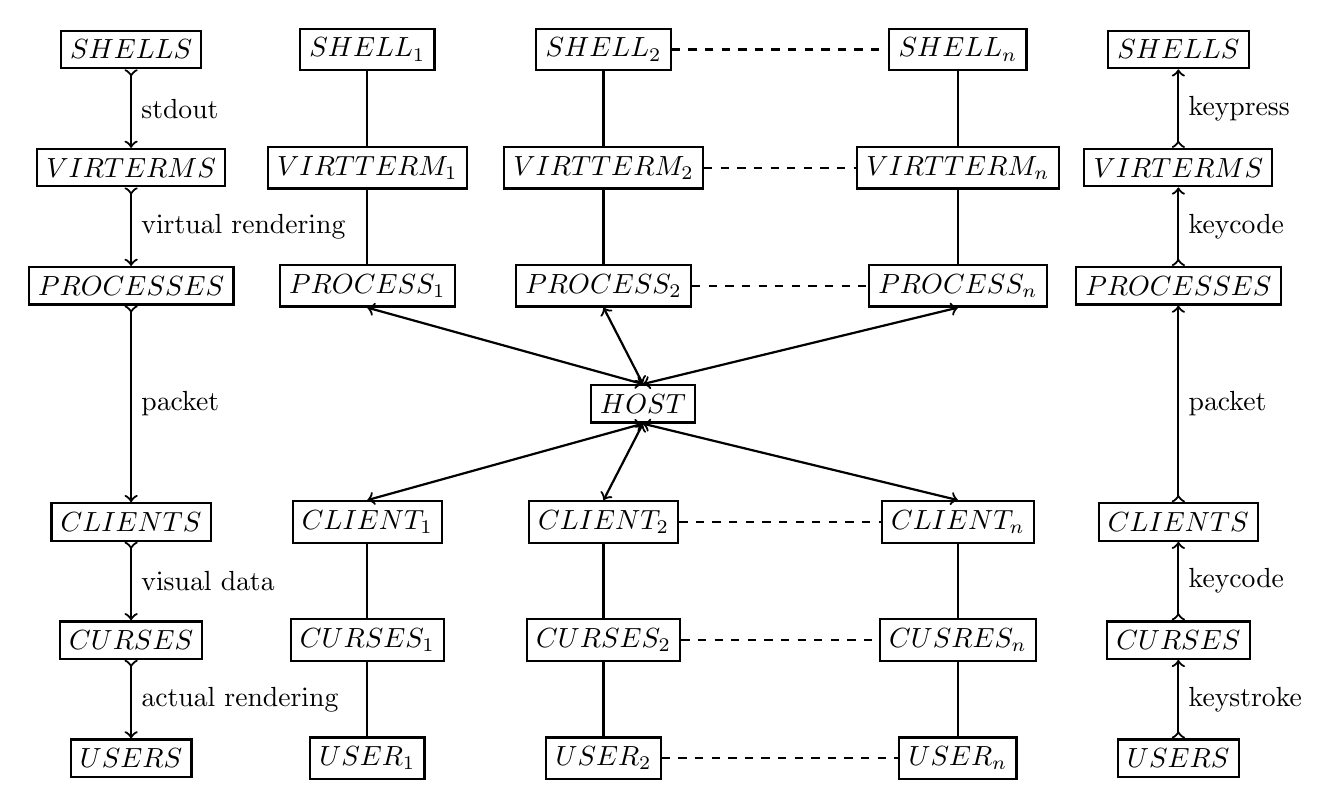
\begin{tikzpicture}[node distance={15mm}, thick, main/.style = {draw, rectangle}]
            \node[main] (HOST) {$HOST$};

            %below the host

            \node[main] (CLIENT1) [below of=HOST, xshift=-3.5cm] {$CLIENT_1$};
            \node[main] (CLIENT2) [below of=HOST, xshift=-.5cm] {$CLIENT_2$};
            \node[main] (CLIENTn) [below of=HOST, xshift= 4cm] {$CLIENT_n$};
            \draw[<->] (HOST) to [out=-90, in=90, looseness=0] (CLIENT1);
            \draw[<->] (HOST) to [out=-90, in=90, looseness=0] (CLIENT2);
            \draw[<->] (HOST) to [out=-90, in=90, looseness=0] (CLIENTn);
            \draw[dashed] (CLIENT2) -- (CLIENTn);

            \node[main] (CL1) [below of=CLIENT1] {$CURSES_1$};
            \node[main] (CL2) [below of=CLIENT2] {$CURSES_2$};
            \node[main] (CLn) [below of=CLIENTn] {$CUSRES_n$}; 
            \draw (CLIENT1) -- (CL1);
            \draw (CLIENT2) -- (CL2);
            \draw (CLIENTn) -- (CLn);
            \draw[dashed] (CL2) -- (CLn);

            \node[main] (US1) [below of=CL1] {$USER_1$};
            \node[main] (US2) [below of=CL2] {$USER_2$};
            \node[main] (USn) [below of=CLn] {$USER_n$}; 
            \draw (US1) -- (CL1);
            \draw (US2) -- (CL2);
            \draw (USn) -- (CLn);
            \draw[dashed] (US2) -- (USn);

            %above the host

            \node[main] (PROCESS1) [above of=HOST, xshift=-3.5cm] {$PROCESS_1$};
            \node[main] (PROCESS2) [above of=HOST, xshift=-.5cm] {$PROCESS_2$};
            \node[main] (PROCESSn) [above of=HOST, xshift= 4cm] {$PROCESS_n$};
            \draw[<->] (HOST) to [out=90, in=-90, looseness=0] (PROCESS1);
            \draw[<->] (HOST) to [out=90, in=-90, looseness=0] (PROCESS2);
            \draw[<->] (HOST) to [out=90, in=-90, looseness=0] (PROCESSn);
            \draw[dashed] (PROCESS2) -- (PROCESSn);
                      
            \node[main] (VT1) [above of=PROCESS1] {$VIRT TERM_1$};
            \node[main] (VT2) [above of=PROCESS2] {$VIRT TERM_2$};
            \node[main] (VTn) [above of=PROCESSn] {$VIRT TERM_n$};
            \draw (PROCESS1) -- (VT1);
            \draw (PROCESS2) -- (VT2);
            \draw (PROCESSn) -- (VTn);
            \draw[dashed] (VT2) -- (VTn);

            \node[main] (SH1) [above of=VT1] {$SHELL_1$};
            \node[main] (SH2) [above of=VT2] {$SHELL_2$};
            \node[main] (SHn) [above of=VTn] {$SHELL_n$};
            \draw (SH1) -- (VT1);
            \draw (SH2) -- (VT2);
            \draw (SHn) -- (VTn);
            \draw[dashed] (SH2) -- (SHn);

            \node[main] (TH) [above of=HOST, xshift=-6.5cm] {$PROCESSES$};
            \node[main] (VT) [above of=TH] {$VIRTERMS$};
            \node[main] (SH) [above of=VT] {$SHELLS$};
            \node[main] (CI) [below of=HOST, xshift=-6.5cm] {$CLIENTS$};
            \node[main] (CL) [below of=CI] {$CURSES$};
            \node[main] (US) [below of=CL] {$USERS$};
            \draw[>->] (SH) -- (VT) node[midway, right] {stdout};
            \draw[>->] (VT) -- (TH) node[midway, right] {virtual rendering};
            \draw[>->] (TH) -- (CI) node[midway, right] {packet};
            \draw[>->] (CI) -- (CL) node[midway, right] {visual data};
            \draw[>->] (CL) -- (US) node[midway, right] {actual rendering};

            \node[main] (TH) [above of=HOST, xshift=6.8cm] {$PROCESSES$};
            \node[main] (VT) [above of=TH] {$VIRTERMS$};
            \node[main] (SH) [above of=VT] {$SHELLS$};
            \node[main] (CI) [below of=HOST, xshift=6.8cm] {$CLIENTS$};
            \node[main] (CL) [below of=CI] {$CURSES$};
            \node[main] (US) [below of=CL] {$USERS$};
            \draw[<-<] (SH) -- (VT) node[midway, right] {keypress};
            \draw[<-<] (VT) -- (TH) node[midway, right] {keycode};
            \draw[<-<] (TH) -- (CI) node[midway, right] {packet};
            \draw[<-<] (CI) -- (CL) node[midway, right] {keycode};
            \draw[<-<] (CL) -- (US) node[midway, right] {keystroke};
        \end{tikzpicture}

        \end{center} 
        This system implements a direct flow of infomation that is encrypted between the host and client, using padding in both directions, and randomized position of actual data for keycodes.\\
        \subsection{Keypair storage}
        The programs store their encryption keys locally to minimize friction, removing the need to generete new ones on each run, but discard the partener's ones as they can be retrieved at any point and are subject to change.
        \section{Implementations}
        \subsection{Instances}
        As shown in the diagram, every client gets one process inside the server's machine which in turn generates a fork where a simulated terminal is created, running the preffered shell of the user as described in their configuration, this is initiated by the following code: 
        \begin{lstlisting}[language=C]    
        while(1){
            if(activeUsers < NUMBER_OF_USERS){
                int pid;
                if((pid = fork()) < 0)
                    error("Forking error", 7);
                if(!pid)
                    instance(&socketFD, &cliLen);
                else{
                    activeUsers += 1;
                    continue;
                }
        }
        \end{lstlisting}
        which checks if it has free slots available and in if it is affirmative it runs an instance described by:
        \begin{lstlisting}[language=C]
    void instance(int * socketFD, socklen_t * cliLen){

        char buffer[BUFFER_SIZE], username[BUFFER_SIZE],keypress;
        
        int newSocketFD;
        newSocketFD = accept(*socketFD, (struct sockaddr *) cliLen, cliLen);
        if(newSocketFD < 0)
            error("socket accept error", 4); 

        bzero(username, BUFFER_SIZE);
        if(read(newSocketFD, username, BUFFER_SIZE) < 0)
            error("Reading error", 5);
       printf("%s",username);

        bzero(buffer, BUFFER_SIZE);
        if(read(newSocketFD, buffer, BUFFER_SIZE) < 0)
            error("Reading error", 5);
        printf("#%s\n", buffer);
    .
    .
    }
        \end{lstlisting}
    taking as input the data required to finish the handshake, and saves the specific socket for communication with its client, then it reads the username and password which will later be used create the PAM authentification method, the password is stored in the general buffer to ensure that it will be deleted as soon as the authentification is complete so even in the case that another process manages to read raw data in the RAM the password not accessible.
    \subsection{Simulated terminal} 
    At the moment of generation of the simulated terminal the server and the client select its size as \\$MIN(SIZE_{MAX}, SIZE_{CLIENT'sTERM})$ which might lead to visual padding of the client's terminal in case it is bigger than it would fit in the buffer. 
    The process takes as input every keypress and actions on it as if it was a keystoke from the server and it outputs every "pixel" equivalent in the terminal so it can be reconstructed.
    \subsection{Actual rendering}
    The client only sends keystrokes to the server (besides the public key, credentials and terminal size) as to allow interactive applications to work continuously on the server's side, and the server sends an complete visual buffer to ensure every part is rendered corectly, this method being required for TUI applications.
    \subsection{Use case}
    This application is useful as a more minimal SSH which can be used when the entire SSH requires more space than there is left on the driver, especially on the client side, as, in virtue of using one direct method, it does not have any redundency in how the communication may happen.

    \section{Conclusion}
    This implementation of a SSH is minimal, it allows for the execution of commands in the server, and permits the continuous observation of the server through a secure connection, although as a disadvantage it imposes CURSES rendering and keystroke detection and RSA encryption.\\
    \\The implementation is fit for purpose, but one way in which it could be improved stands out, which is detecting the keystrokes at a lower level (thus making signal sending more purposeful, since in this implementation every signal is passed to the server, and ignored on the client, ignoring its source as intended behaveour). \\
    \\Other ways in which the implementation could be improved is rendering the clientside application at a lower level, but it would require multiple implementations to pretain to different terminals as even though ANSI escape codes are standard they are not maintained in many third party terminal emulators, \\
    and implementing multiple possible encryption methods that could be switched inside the $config.h$ file by defining the encryption method at compile.

    \section{References}
    \sf 1. What is an SSH as defined as the standard SSH: \bf\href{https://manpages.org/ssh}{https://manpages.org/ssh} \\
    \sf 2. What is TCP: \bf\href{https://manpages.org/tcp/4}{https://manpages.org/tcp/4} \\
    \sf 3. How does the TCP handshake work:  \bf\href{https://www.guru99.com/tcp-3-way-handshake.html}{https://www.guru99.com/tcp-3-way-handshake.html} \\
    \sf 4. How RSA works: \bf\href{https://www.simplilearn.com/tutorials/cryptography-tutorial/rsa-algorithm}{https://www.simplilearn.com/tutorials/cryptography-tutorial/rsa-algorithm} \\
    \sf 5. What is PAM and how it works: \bf\href{https://linux.die.net/man/8/pam}{https://linux.die.net/man/8/pam} \\

\end{document}
